%   This file is part of the AIP files in the AIP distribution for REVTeX 4.
%   Version 4.1 of REVTeX, October 2009
%
%   Copyright (c) 2009 American Institute of Physics.
%
%   See the AIP README file for restrictions and more information.
%
% TeX'ing this file requires that you have AMS-LaTeX 2.0 installed
% as well as the rest of the prerequisites for REVTeX 4.1
%
% It also requires running BibTeX. The commands are as follows:
%
%  1)  latex  aipsamp
%  2)  bibtex aipsamp
%  3)  latex  aipsamp
%  4)  latex  aipsamp
%
% Use this file as a source of example code for your aip document.
% Use the file aiptemplate.tex as a template for your document.
\documentclass[%
 aip,
 jmp,%
 amsmath,amssymb,
%preprint,%
reprint,%
%author-year,%
%author-numerical,%
]{revtex4-1}
\usepackage[utf8]{inputenc}
\usepackage{amsmath}  % needed for \tfrac, \bmatrix, etc.
\usepackage{amsfonts} % needed for bold Greek, Fraktur, and blackboard bold
%\usepackage{graphicx} % needed for figures

\usepackage[pdftex]{graphicx}% Include figure files
%\usepackage{tabularx}
%\usepackage{bm}% bold math
\usepackage{epstopdf}
\usepackage{siunitx}
\usepackage{xcolor}
\usepackage{algpseudocode}
\usepackage[pdftex=true,colorlinks=true,linkcolor=blue,citecolor=blue]{hyperref}
\usepackage[all]{hypcap} %% Sans ce package, lorsqu'on clique sur un lien menant à une image, ça ne mène pas au bon endroit
%\usepackage{booktabs}
\epstopdfsetup{outdir=./epstopds_converted/}
%\usepackage[mathlines]{lineno}% Enable numbering of text and display math
%\linenumbers\relax % Commence numbering lines
\newcommand*\circled[1]{\raisebox{0.5pt}{\textcircled{\raisebox{-.9pt} {#1}}}}
%\newcommand{\hh}{\\ \vspace{0.1cm} \\}
%\graphicspath{{C:/thomas/research/david/Article/epstopds_converted}}
%\graphicspath{{epstopds_converted}}


\begin{document}

\preprint{AIP/123-QED}

\title[Differential Dynamics Microscopy to characterize Brownian motion and bacteria motility]{Differential Dynamics Microscopy\\ to characterize Brownian motion and bacteria motility}% Force line breaks with \\

\author{David Germain}
\author{Mathieu Leocmach}
\author{Thomas Gibaud}
\affiliation{Universit\'e de Lyon, Laboratoire de Physique, \'Ecole Normale Sup\'erieure de Lyon, CNRS UMR 5672, 46 All\'ee d'Italie, 69364 Lyon cedex 07, France}

\date{\today}% It is always \today, today,
             %  but any date may be explicitly specified

\begin{abstract}
Quantifying the dynamics of a suspension of microscopic particles consists in measuring and analyzing the motion of those particles at the individual level or as a group.  Differential Dynamic Microscopy (DDM) precisely does that and constitutes an alternative method to more classical techniques such as dynamics light scattering (DLS) or video particle tracking (VPT). DDM consist in imaging a particle dispersion with a standard light microscope and a camera. The image analysis requires to code and  relies on digital Fourier transform to obtain the intermediate scattering function, an autocorrelation function that characterizes the dynamics of the dispersion. We illustrate DDM on two sets of dispersions, colloids and motile bacteria. We have joined to this article movies of the  colloidal and bacterial suspensions and the DDM code in matlab and python so that the reader may reproduce the image analysis proper to DDM.
\end{abstract}

\pacs{42.30Va -- 87.17.Jj -- 82.70.Dd -- 87.80}% PACS, the Physics and Astronomy
                             % Classification Scheme.
\keywords{Dynamics, Bacteria, Colloid, Microscopy, Intermediate Scattering Function, Image Analysis}%Use showkeys class option if keyword
                              %display desired
\maketitle

\section{\label{sec:level1}Introduction}

Quantifying the dynamics of a suspension of microscopic particles consists in measuring and analyzing the motion of those particles at the individual level or as a group. Like hockey for Canadians or cricket for Indians and Pakistanis, quantifying the dynamics of a suspension of microscopic particles is the national sport of a large community of researchers in physics and biology. For example, a century ago, Perrin has characterized the motion of small particles in a liquid, an experiment that evidenced the Brownian motion and firmly proved the existence of atoms \cite{22_perrin2014atomes}. More recently, the motion of tracer particles has been used to extract the mechanical properties such as viscosity or elasticity of fluids, gels\cite{Mason1997, Chen2010}, pastes, cell cytoplasm\cite{Fabry2001,Lau2003} and foods at scales unreachable by macroscopic techniques. In the past decade, the study of the collective motion of fish schools, bird flocks and bacteria swarms has lead to the emergence of a new field, active matter \cite{Bricard2013}.

Video Particle Tracking (VPT) and Dynamic Light Scattering (DLS) are two of the most well-known techniques that allows to characterize the dynamics of a suspension of microscopic particles. VPT consists in tracking the position of an individual particle as a function of time to digitalize its trajectory. It provides precise information of small portions of a sample \citep{7_jaqaman2008robust}. DLS consists in shining a laser through the particle suspension and monitoring the fluctuations of scattered intensity as a function of time. It yields average information about the dynamics of a sample \citep{18_sartor2003dynamic}.

Here, we describe an alternative method called Differential Dynamic Microscopy (DDM) recently proposed by Cerbino and Trappe \cite{2_DDM}. DDM is intuitive as it deals with real-space video of the moving objects like VPT, however it uses digital Fourier transform to obtain the same kind of information as DLS.  Contrary to tracking algorithm DDM algorithm is straightforward to implement at the programming level of most undergraduate students. We believe lab work on DDM is a great opportunity to become familiar with a microscope and with reciprocal units, the range of accessible wavenumbers and other nitty-gritty details necessary to tame the power of the Fourier transform. We have joined to this article movies of suspensions with different types of particles and the DDM codes so that the reader may reproduce the image analysis proper to DDM, see EPAPS.

In this article, we apply DDM to two sets of different micrometer particles, colloids at first, then motile bacteria. In section \ref{materials}, we present the materials and method we used to prepare the samples as well as the acquisition parameters. In section \ref{sec:BrownSection}, we use the Brownian motion of colloids as a support to present step by step DDM in a fully understood context. In a last part, section \ref{sec:BactSection}, we apply DDM to \textit{salmonella} bacteria and show that it is possible to characterize entangled dynamics where the bacteria both diffuse and ``swim".

\section{Materials and methods}
\label{materials}
\subsection{Colloidal particles}

As colloids, we use polystyrene spheres with a catalog radius of $R=\SI{0.50}{\micro\meter}$  (FluoSpheres\circledR{} from Thermo Fisher Scientific). The commercial dispersion is diluted 50 times in water to a final concentration of $\SI{1e8}{colloids\per\milli\liter}$ so that we have a dilute dispersion: the distance between two colloids is large compared to $R$, typically $20 R$. This concentration remains sufficiently high to observe enough particles in the camera field of view and to accumulate decent statistics.

Polystyrene refractive index is $\approx 1.6$, larger than the one of water $\approx 1.3$, so the colloids are visible in bright field microscopy. However cleaner images can be obtained by fluorescence microscopy, exiting at \SI{540}{\nano\metre} and filtering to obtain the emitted light at \SI{560}{\nano\metre}.

\subsection{Bacteria}
In section \ref{sec:BactSection}, we study the motion of \textit{Salmonella} bacteria (DSM. 1103) \citep{21_fabrega2013salmonella}. Our bacteria are stored in a freezer at $\SI{-80}{\degree C}$ in a mixture of water ($\simeq \SI{33}{\%}$) and glycerol ($\simeq \SI{66}{\%}$). First, using a sterile inoculation loop, we streak bacteria from the storage solution on a sterile agar/LB plates  ($\SI{500}{\milli\liter}$ of LB/agar was made of $\SI{5}{\gram}$ of NaCl, $\SI{5}{\gram}$ of Tryptone, $\SI{2.5}{\gram}$ of Yeast Extract, $\SI{7.5}{\gram}$ of Agar). Second, the agar plates are closed and placed in an incubator at $\SI{37}{\degree C}$. The agar plates are oriented such that the LB/agar gel is at the top, to prevent the condensation from disturbing the development of the bacteria. After $\simeq$ 12 hours, we observe the formation of monoclonal circular colonies. Third, Using an inoculation loop, we take a monoclonal colony of bacteria from LB/Agar plate and disperse it in a \textsc{Falcon} tube with $\simeq \SI{5}{\milli\liter}$ TN growth medium. The TN growth medium is sterile and composed of $\SI{4}{\gram\per\liter}$ of bacto-tryptone, $\SI{2.5}{\gram\per\liter}$ of NaCl and $0.4\%$ of glycerol diluted in water. The \textsc{Falcon} tubes have an oxygen permeable cap which allows the bacteria to breath and limits evaporation. Those bacteria are pre-cultured for a night at $\SI{32}{\degree C}$ and shaked at 300 rpm in an Incu-Shaker 10L. Finally, we collected $\SI{50}{\micro\liter}$ of the solution of bacteria with a sterile pipette and we put it in a new \textsc{Falcon} tube filled with $\simeq \SI{5}{\milli\liter}$ of TN growth medium. The tube is then placed in the Incu-Shaker 10L at 300 rpm and $\SI{32}{\degree C}$ for 1h30. Around this time the optical density (OD) at $\SI{600}{\nano\meter}$ is around OD=0.5 and most bacteria are ``swimming". It is important to grow bacteria in a nutriment poor media and to collect them early on, at low concentrations, otherwise the bacteria tend not to develop a flagella. More details about bacteria preparation can be obtained in ref\cite{Schwarz2015}.

\subsection{Microscope slide}
For the microscope observations, the aqueous suspension of colloids or bacteria are enclosed in a home made hermetic optical cell, Fig.\ref{Slide}.a. The cell is composed of a  glass slide (\textsc{RS France}) and a cover slip (\textsc{Menszel-gl\"aser}) spaced by two stripes of paraffin film (\textsc{Bemis}). The optical cell is briefly heated on a hot plate so that the paraffin welds to the slide and the cover slip. The space between the glass slide and the cover slip is approximately $\SI{125}{\micro\meter}$. The suspension of colloids or bacteria is then introduced into the slit by capillarity, and the cell is immediately sealed using ultraviolet-cured glue (Norland Optical).

%fig 1%%%%%%%%%%%%%%%%%%%%%%%%%%%%%%%%%%%%%%%
\begin{figure}
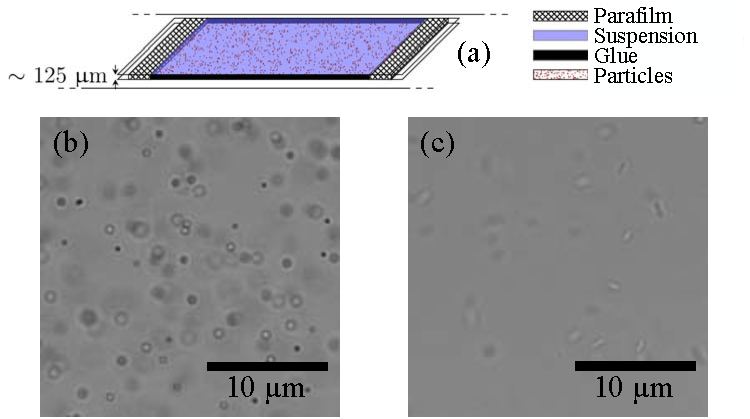
\includegraphics[width=\linewidth]{Lamelle_Photos.pdf}
\caption{Experimental setup. (a) Schematics of the microscope cell used to study the motion of particles, namely, colloids and bacteria. (b) Detail of a typical bright field image of our colloidal suspension. (c) idem with bacteria.}
\label{Slide}
\end{figure}

\subsection{Microscope and acquisition parameters}

The colloidal and bacterial suspensions are observed with light microscope (\textsc{nikon Eclipse Ti}) in transmitted visible light with an objective $10 \times$ of numerical aperture $N.A. = 0.3$, Fig.\ref{Slide}.b-c. The focus is made in the middle of the microscope slide in $z$-direction. It allows to be far from the boundaries where colloids could be stuck on the slide and could not move in the 3 dimensions. Images are acquired with a camera (\textsc{Hamamatsu ORCA-Flash2.8}).

The images are coded in $\SI{8}{bits}$  grey-scale: each pixel intensity is proportional to the incoming light intensity from the sample and varies linearly from  0 (black) to 255 (white). Using an exposure time of $\SI{1}{\milli\second}$, we adjusted the brightness of the microscope light in order to have a maximum number of pixel around a value of $\sim 120$ which minimize the amount of saturated pixels.

The choice of the acquisitions parameters is a compromise between the spatial and the temporal resolution. With the $10\times$ objective, a pixel corresponds to $\SI{0.645}{\micro\meter}$, a bit smaller than the optical resolution of the microscope, $\lambda/(2N.A.)\approx\SI{0.8}{\micro\meter} $. Bacteria or colloids are about $\SI{1}{\micro\meter}$ and therefore correspond to a few pixels on the camera. We chose a $(\SI{512}{px})^2$ field of view which is large enough to capture the motion of 100 of particles and small enough to reach high acquisition frequencies, up to $\SI{400}{\hertz}$. At $\SI{400}{\hertz}$ it is impossible to directly sent the data from the camera to the computer during the capture, so we have to temporarily save the acquisition on the buffer of the camera, and, once it is over, we send the data from the buffer of the camera to the computer. The camera buffer memory limits the number of images in one stack to 4000. To cover a wide range of time scales, we chose to acquire a first stack of 4000 images at $\SI{400}{\hertz}$ and a second similar stack at $\SI{4}{\hertz}$. With this procedure, we cover time scales between $\SI{2.5e-3}{\second}$ and $\SI{1000}{\second}$ and length scales between $\SI{0.645}{\micro\meter}$ and $\SI{330}{\micro\meter}$.

\section{Brownian motion and DDM}
\label{sec:BrownSection}

\subsection{The Brownian motion}

The Brownian motion is the unceasing and random motion of small particles suspended in a fluid at rest. Brownian motion has a particularly interesting history. It has been observed since the 18th century, and maybe even before. Robert Brown, a Scottish botanist from the beginning of the 19th century, who was interested in the action of pollen on plant reproduction, observed the irregular and unceasing motion of micrometer particles in the internal fluid of grain of pollen \citep{13_brown1828brief}. At the time, such microscopic agitation was seen as \textit{a priori} a biological phenomenon. Nevertheless, R. Brown showed that this phenomenon persist with inorganic particles, refuting the wrong concept based on living particles. It's only at the beginning of the 20th century that physicists could interpret and analyze the Brownian motion. The particularity of the Brownian motion which has prevented every attempt of interpretation in the 19th century, is that the particle dynamics is perpetual, unlike other usual experiments where friction eventually stop the motion. Albert Einstein \citep{9_einstein1906theory}, William Sutherland \citep{14_sutherland1905lxxv}, Marian von Smoluchowski \citep{10_von1906kinetischen} and Paul Langevin \citep{15_Langevin} explained Brownian motion using the atomic hypothesis, i.e. that the fluid is not a continuous medium but is composed of individual molecules far smaller than the Brownian particles. They demonstrated that it is the shocks between the molecules of the liquid and the Brownian particles that are at the origin of the Brownian motion. This assumption has been validated by the experiments made by Jean Perrin in 1928 \citep{22_perrin2014atomes}. With a microscope and photographs, the team of Jean Perrin reconstructed ``by hand" the trajectories of Brownian particles and deduced a correct measure of the Avogadro constant, validating the theory of Brownian motion and therefore the atomic hypothesis.

\subsection{Colloidal particles}

To observe the Brownian motion of particles in a Newtonian fluid, several conditions are required \citep{16_CollSusp}. The particle has to be colloidal, meaning that its size has to be far larger than the size of the solvent molecules, it is the case for the suspension we used, see Table \ref{TabParams}. Furthermore, colloidal particles have to be in the dilute regime to avoid interaction between them. This is checked once the sample is made. As our colloids do not have long distance interaction, we estimate that the sample is dilute when the mean distance between colloids is higher than at least 10 times the diameter of a colloid. Finally, one has to make sure that the thermal agitation is the physical process that dominates the dynamics of the colloidal particles. We ensure that the solvent is not flowing by using an immobile, sealed and thin optical cell with negligible temperature gradient. The sedimentation motion can be characterized by the P\'eclet number \citep{12_patankar1980numerical}
\begin{equation}
\text{Pe}_\text{g} = \frac{E_\text{g}}{E_\text{th}},
\end{equation}
where $E_\text{g} = \frac{4 \pi R^3}{3}  (\rho_\text{c} - \rho_\text{s}) g  2R$ is the variation of potential energy for a difference of altitude equal to the diameter $2R$ of the particle, $E_\text{th} = k_\text{B} T$ is the thermal energy, $\rho_\text{c}$ and $\rho_\text{s}$ the respective densities of the particle and the surrounding solution, $g$ the acceleration of gravity, $k_\text{B}$ the Boltzmann constant and $T$ the temperature. Here we have $\text{Pe}_\text{g} \approx 0.1$, indicating that the sedimentation can be neglected over Brownian motion. Equivalently in the time domain, our colloid sediments and diffuses on a distance equal to its own diameter on a characteristic time $\tau_\text{s}=9\eta/(8(\rho_\text{c}-\rho_\text{s}) R)\approx$ 100 s for sedimentation much larger than the characteristic time $\tau_\text{d}=24\pi\eta R^3/k_BT\approx$2 s for diffusion. Absence of both flow and sedimentation will be verified \textit{a posteriori}. In presence of a flow the trajectory of the colloid, normally random, is biased in the direction of the flow.

\begin{table}
\begin{tabular}{m{0.7\linewidth}m{0.28\linewidth}}
  \hline\\[-0.8em]
  Molecular diameter of water \citep{17_marcus1998properties}  & $\SI{0.34}{\nano\meter}$\\
  Temperature $T$ of the suspension & $\SI{20}{\degree C}$ \\
  Tabulated viscosity of water at $T$, $\eta$ & $\SI{1.002}{\milli\pascal\second}$ \\
  Density of polystyrene, $\rho_\text{c}$ & $\SI{1.04}{\gram\per\centi\meter\cubed}$ \\
  Density of water, $\rho_\text{s}$ & $\SI{1.00}{\gram\per\centi\meter\cubed}$ \\ 
  Colloid diameter, $2R$ & $\SI{1}{\micro\meter}$\\
  \hline
  \end{tabular}
  \caption{Properties of colloidal particles and their medium}
  \label{TabParams}
\end{table}

\subsection{Stokes-Einstein relation}

The Brownian motion is random with the same probability to move in any direction after a collision, the average position of a particle do not carry any physical information. Instead the relevant length scale is the mean square displacement \citep{11_ken2003molecular} $\langle \Delta r^2(\Delta t) \rangle$. By resolving the equation of diffusion for a density $\rho(\vec{r}, t)$ of Brownian particles, it can be shown \cite{9_einstein1906theory} that the second moment of $\rho(\vec{r}, t)$ is:
\begin{equation}
\left\langle \Delta r^2(\Delta t) \right\rangle = 2dD \Delta t
\label{eq:msd}
\end{equation}
where $d$ is the dimension of the space and $D$ is the diffusion coefficient. As predicted by theory, our experiment \cite{Maurer2014} shows that the mean square displacement scales linearly with time, Fig. \ref{BrownianTrajectory}.b. This scaling is one of the hallmark of a diffusive process; if the motion was ballistic, we would observe $\left\langle \Delta r^2(\Delta t) \right\rangle \sim \Delta t^2$.

%fig 2%%%%%%%%%%%%%%%%%%%%%%%%%%%%%%%%%%%%%%%
\begin{figure}
	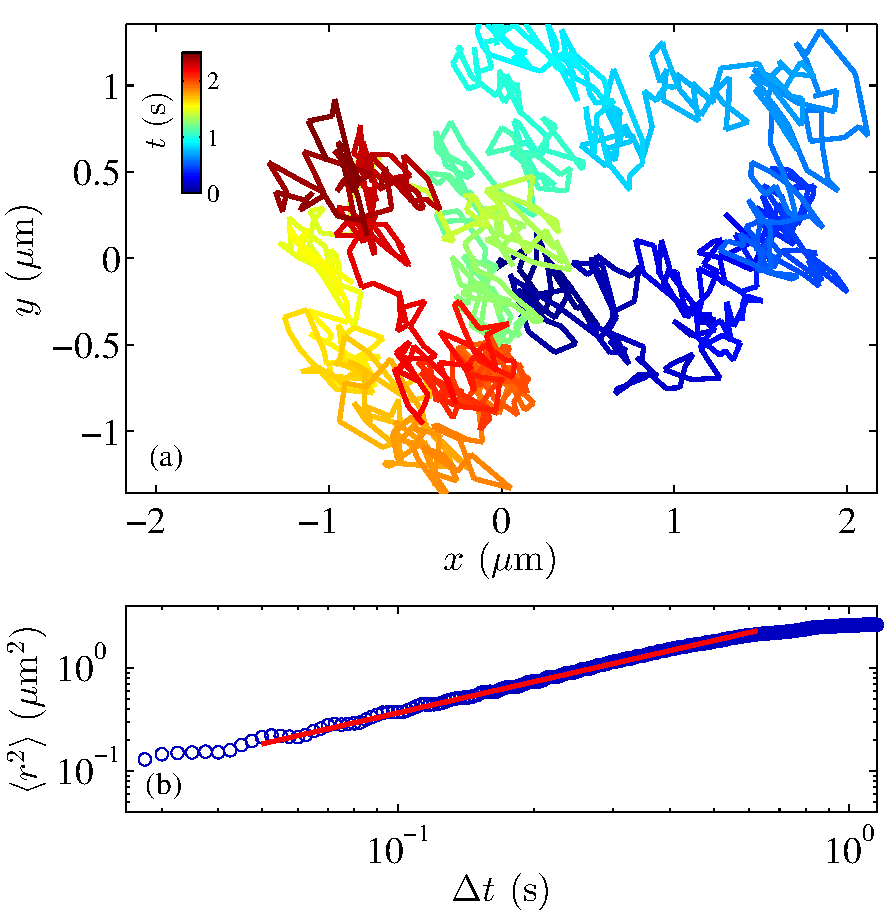
\includegraphics[width=\linewidth]{BrownianPres.pdf}\\
	\caption{(a) Trajectory of a brownian particle obtained by particle tracking as a function of time. Positions of a colloid of diameter 1 $\mu$m in an aqueous suspension at various times from $t=0$ s (blue) to $t=2.5$ s (red). The time increment is $2.5 \times 10^{-3}$ s. (b) Mean Square Displacement of the colloid as a function of $t$ calculate from the trajectory in (a). }
	\label{BrownianTrajectory}
\end{figure}

An other way to look at the dynamics of the system is to forget about individual trajectories but rather quantify the evolution of the system during the time interval $\Delta t$. Formally, we can define an auto-correlation function $f(\Delta t)$ whose value goes from 1 when the system has not changed ($t=0$) to 0 when the system has changed completely $(t\rightarrow\infty)$. In Fig. \ref{SketchCorrelation}, we have superimposed two images of a colloidal dispersion separated by a lag time $\Delta t$. At $\Delta t = \SI{0.01}{\second}$, the colloids have barely moved and $f \simeq 1$. At $\Delta t = \SI{1}{\second}$, the colloids have moved and we can identify where they have come from.  At $\Delta t = \SI{100}{\second}$, the colloids have moved so much that we no longer know where they have come from and $f \simeq 0$: the two images are totally decorrelated.

%fig 3%%%%%%%%%%%%%%%%%%%%%%%%%%%%%%%%%%%%%%%
\begin{figure}
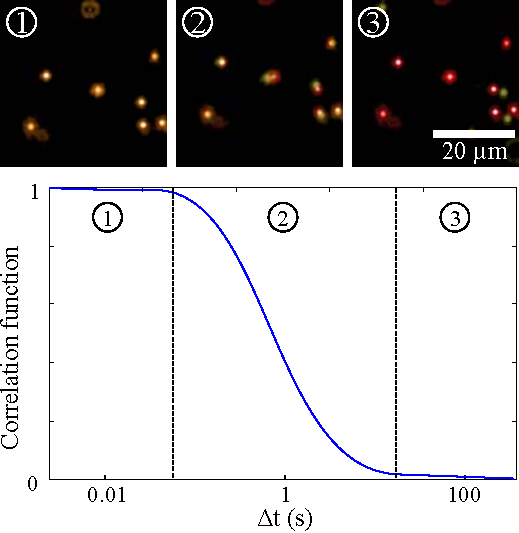
\includegraphics[width=\linewidth]{ComparaisonImage.pdf}
\caption{Differential Dynamic Microscopy (DDM) principle. Superpositions of 2 images of a colloidal dispersion taken at various intervals of time and sketch of the correlation function. Each picture is composed of 2 images, the first one is colored in yellow and taken at $t = 0$ s, the other is colored in red and taken at $t = \Delta t$. \protect\circled{1}: $\Delta t = 0.01$ s; \protect\circled{2}: $\Delta t = 1$ s; \protect\circled{3}: $\Delta t = 100$ s. Correlation function between 2 sets of positions associated with each pictures. At low $\Delta t$, the 2 sets are very correlated \protect\circled{1} and the correlation function is 1. For $\Delta t \sim 1$ s, the correlation decrease \protect\circled{2}. For long $\Delta t$, the 2 sets are almost completely decorrelated \protect\circled{3} and the correlation function is 0.}
\label{SketchCorrelation}
\end{figure}

The auto-correlation function depends on the length scale: a smaller field of view will appear decorrelated faster. This is more readily expressed in Fourier space by the wavenumber $q$, so that we have $f(q, \Delta t)$ for $\tau \sim 1$. This $q$ dependance of the auto-correlation function allows us to determine the physical origin of the decorrelation process. For balistic particles, the characteristic decorellation time $\tau$ necessary to advect a density is  proportional to the distance $2\pi/q$ whereas, for diffusive particles, the characteristic decorellation time $\tau$ necessary to diffuse a density is proportional to $(2\pi/q)^2$. Here we drop the dependence on the orientation of the wavevector $\vec{q}$ since we are dealing only with isotropic systems. 

We can get quantitative information about the dynamics of the sample either by scaling the correlation function or by fitting the correlation with a model. For a stochastic process such as the Brownian motion, the decrease of the correlation function is exponential : $f(q, \, \Delta t) = \exp(-\Delta t/\tau_\text{d})$, with $\tau_\text{d}$ the characteristic time of the decay \citep{8_berne2000dynamic}. Equivalently to (Eq.~\ref{eq:msd}), time and space variables are related by
\begin{equation}
\tau_\text{d} = \frac{1}{Dq^2}.
\label{eq:relax}
\end{equation}

The diffusion coefficient $D$, common to (Eq.~\ref{eq:msd}) and (Eq.~\ref{eq:relax}), is increasing with the temperature and decreasing with the radius $R$ of the particle and the viscosity $\eta$ of the fluid according to the \textsc{Stokes-Einstein} formula \citep{9_einstein1906theory}:
\begin{equation}
D = \frac{k_\text{B} T}{6 \pi \eta R}
\end{equation}

\subsection{Differential Dynamics Microscopy}

Dynamic Light Scattering (DLS) and Differential Dynamics Microscopy (DDM) are two different ways to obtain the auto-correlation function of a stationary system, that is to say a system whose statistical properties does not change when shifted in time. In DLS we measure the intensity $\hat{I}$ scattered by the sample at a given angle, i.e at a given wavenumber $q$ in the Fourier space. Time autocorrelation of this signal yields the so called Intermediate Scattering Function (ISF)~\citep{19_goodman2005introduction} $F(q, \, \Delta t) = \left\langle \hat{I}^*(\vec{q}, t) \hat{I}(\vec{q}, t+\Delta t) \right\rangle$, where brackets denote the average over the initial time $t$ and the orientation of the wavevector $\vec{q}$. The ISF is normalized into $f$ by
\begin{equation}
f(q, \Delta t) = \frac{F(q, \Delta t)}{F(q, 0)}.
\end{equation}

In DDM, we acquire microscopy images in real space as $I(\vec{r}, t)$ and then digitally processed them to obtain $f(q, \Delta t)$ as follow. We consider the difference between two images separated by $\Delta t$,
\begin{equation}
\Delta I(\vec{r},t, \Delta t) = I(\vec{r}, t+\Delta t) - I(\vec{r}, t)
\end{equation}
and we compute numerically its spatial 2D Fourier transform $\widehat{\Delta I}$. Once ensemble averaged, the squared normed of this quantity is directly related to the correlation function, thanks to the cross product term:
\begin{align*}
\mathcal{D}(q,\Delta t) \equiv& \left\langle \left|\widehat{\Delta I}\right|^2 \right\rangle\\
 =& \left\langle \left|\widehat{I}(q,t+\Delta t) - \widehat{I}(q,t)\right|^2 \right\rangle \\
=& \left\langle \left|\widehat{I}(q,t+ \Delta t)\right|^2 + \left|\widehat{I}(q,t)\right|^2\right. \\
&\left.- 2 \, \widehat{I}^*(q,t+\Delta t) \widehat{I}(q,t) \right\rangle\\
=& \underbrace{2F(q, 0)}_{\equiv A(q)} \bigg[ 1-\underbrace{\frac{F(q, \Delta t)}{F(q, 0)}}_{f(q, \Delta t)} \bigg]\\
\end{align*}

The contribution of the noise due to the camera is taken into account by adding a supplementary term $B(q)$. $B(q)$ is decorrelated  at all time and therefore independent of $\Delta t$.

\begin{equation}
\mathcal{D}(q,\Delta t) = A(q)\left[1-f(q, \Delta t)\right] + B(q)
\label{eq:D2f}
\end{equation}

The parameters $A(q)$ and $B(q)$ can be used as fitting parameters or measured independently thus giving access directly to the correlation function. The range of accessible $q$ depends on both the image size and the pixel size.

In Fig.\ref{DifferenceAndFFT} we show $I(\vec{r}, t)- I(\vec{r}, t+\Delta t)$ and the corresponding power spectrum for increasing value of $\Delta t$. As $\Delta t$ increases, colloids move more and the difference between two images shows a growing signal on larger and larger length scale. The power spectra are isotropic and as $\Delta t$ increases a peak appears at a wave vector which correspond to the most probable distance between two colloids.

%fig 4%%%%%%%%%%%%%%%%%%%%%%%%%%%%%%%%%%%%%%%
\begin{figure*}
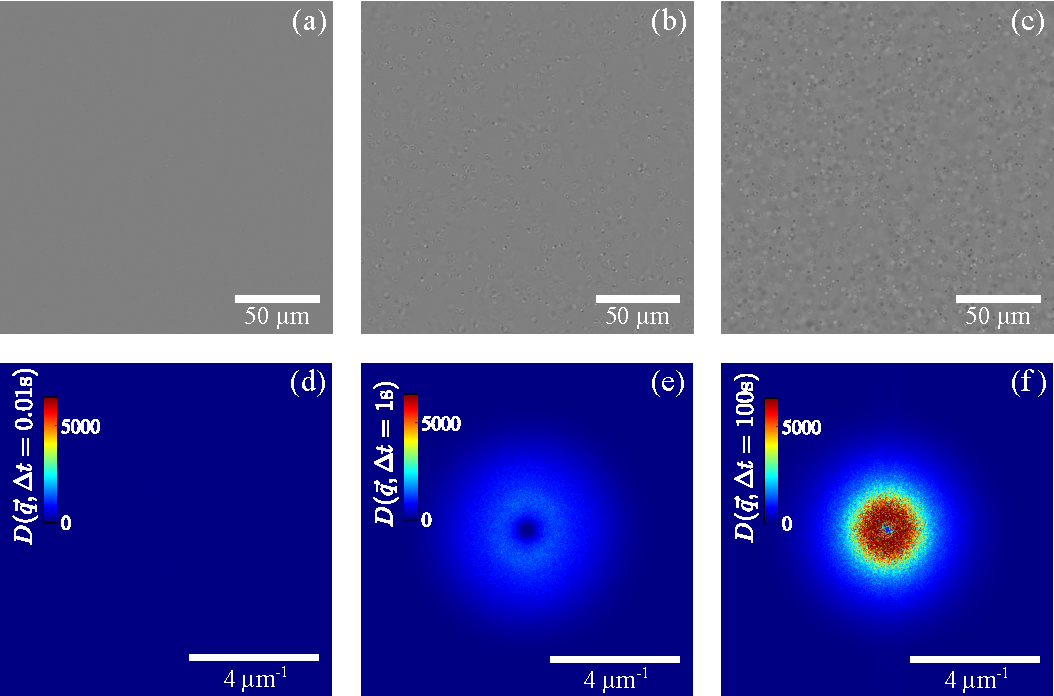
\includegraphics[width=\linewidth]{Diff_TF.pdf}
\caption{Image differences of a colloidal suspension and their Fourier transform as a function of $\Delta t$. (a, b, c) Differences between 2 images separated by $\Delta t$. (d, e, f) 2D Fourier transforms of those differences. These differences and Fourier transforms are calculated with $\Delta t = 0.01$ s (a, d), $\Delta t = 1$ s (b, e), $\Delta t = 100$ s (c, f). The unit of the Fourier transforms is arbitrary.}
\label{DifferenceAndFFT}
\end{figure*}

Implementations of Fast Fourier Tranform (FFT) algorithms are widespread and included in most high-level languages. However, we note that the calculation time necessary to compute all the FFT at all the accessible $\Delta t$ can become very long (some hours). To alleviate this burden, we sample $\Delta t$ logarithmically with 10 points per decades. Furthermore, for each $\Delta t$ we use at most 100 couples of images selected so that the initial times are evenly spread across the accessible time window. This is sufficient to obtain isotropic Fourier spectra that we average radially. With those optimizations, the calculation time falls to a few minutes.

We ran the DDM procedure on both stacks of images at $\SI{400}{\hertz}$ and $\SI{4}{\hertz}$ independently. Then the we merged the two sets of data by scaling the data at $\SI{4}{\hertz}$ so that both values at \SI{0.25}{\second} are equal. Finally, we average the values of the curves at $\SI{4}{\hertz}$ and $\SI{400}{\hertz}$ in the overlap interval, from $\SI{0.25}{\second}$ to $\SI{10}{\second}$. We obtain $\mathcal{D} (q, \Delta t)$ for $\Delta t$ from $\SI{2.5e-3}{\second}$ to $\SI{1000}{\second}$. The DDM procedure is summarized in Table \ref{AlgoTable}.

\begin{table}
\begin{tabular}{ |p{0.98\linewidth}| }
  \hline
  \\  
  Two acquisitions:
  \begin{itemize}
  \item 4000 images $I(\vec{x},t)$ per acquisitions
  \item Acquisiton 1 : $f_{acq}=\SI{400}{\hertz} \rightarrow t_\text{max} = \SI{10}{\second}$
  \item Acquisiton 2 : $f_{acq}=\SI{4}{\hertz} \rightarrow t_\text{max} = \SI{1000}{\second}$
  \item Exposition time = $\SI{1}{\milli\second}$
  \item Image size = $(\SI{512}{px})^2$
  \end{itemize}
  \\
  \hline
  \\
  DDM algorithm:
  \begin{algorithmic}[0]
  	\For{$\Delta t = 1/f_{acq} \rightarrow t_\text{max}$ in log scale}
  		\For{at most 100 values of $t\in[0, t_\text{max}- \Delta t]$}
  			\State $\Delta I(\vec{x},t,\Delta t) \gets I(\vec{x},t+\Delta t) - I(\vec{x},t)$
  			\State $|\widehat{\Delta I}(\vec{q},t,\Delta t)|^2 \gets |\text{FFT}[\Delta I(\vec{x},t,\Delta t)]|^2$
  		\EndFor
  		\State $\langle |\widehat{\Delta I}|^2 \rangle (\vec{q}, \Delta t) \gets $ average on $t$
  	\EndFor
  	\State $ \mathcal{D}(q,\Delta t)=\langle \, |\widehat{\Delta I}|^2 \, \rangle (q, \Delta t) \gets$ radial average 
  \end{algorithmic}
  \\
  \hline
\\
  Recovering the intermediate scattering function, $f$:
  \begin{itemize}
  \item $\mathcal{D}(q,\Delta t) = A(q)\left[1-f(q, \Delta t)\right] + B(q)$
 \item $A$ and $B$ are experimental parameters.
\item Scale and fit $f$ with the appropriate model.
  \end{itemize}\\
  \\
  \hline
\\
  Length scales:
  \begin{itemize}
  \item $\SI{1}{px} = \SI{0.645}{\micro\meter}$
  \item $q_\text{min} = \frac{2 \pi}{0.645 \times 512} = \SI{1.9e-2}{\per\micro\meter}$
  \item $q_\text{max} = \frac{512}{2} q_\text{min} = \SI{4.9}{\per\micro\meter}$
  \end{itemize}
\\
  \hline
\end{tabular}
\caption{Summary of the DDM procedure.}
\label{AlgoTable}
\end{table}

\subsection{Results}

In Fig.\ref{D}, $\mathcal{D}(q, \Delta t)$ is plotted as a function of $q$ for various $\Delta t$ and as a function of $\Delta t$ for various $q$. For small $\Delta t$  as shown in Fig.\ref{D}.b, we observe a first plateau. Images are very correlated, colloids didn't move enough between two images separated by $\Delta t$ and the colloids motion is barely visible on the differences between the images. Thus $f(q, \Delta t) \simeq 1$, and according to (Eq.~\ref{eq:D2f}) we only observe the contribution of the noise $B(q)$. For large $\Delta t$, we observe a second plateau at a higher value because the images are completely decorrelated, $f(q, \Delta t) \simeq 0$ thus $\mathcal{D}(q, \Delta t) \simeq A(q)+B(q)$.

%fig 5%%%%%%%%%%%%%%%%%%%%%%%%%%%%%%%%%%%%%%%
\begin{figure}
	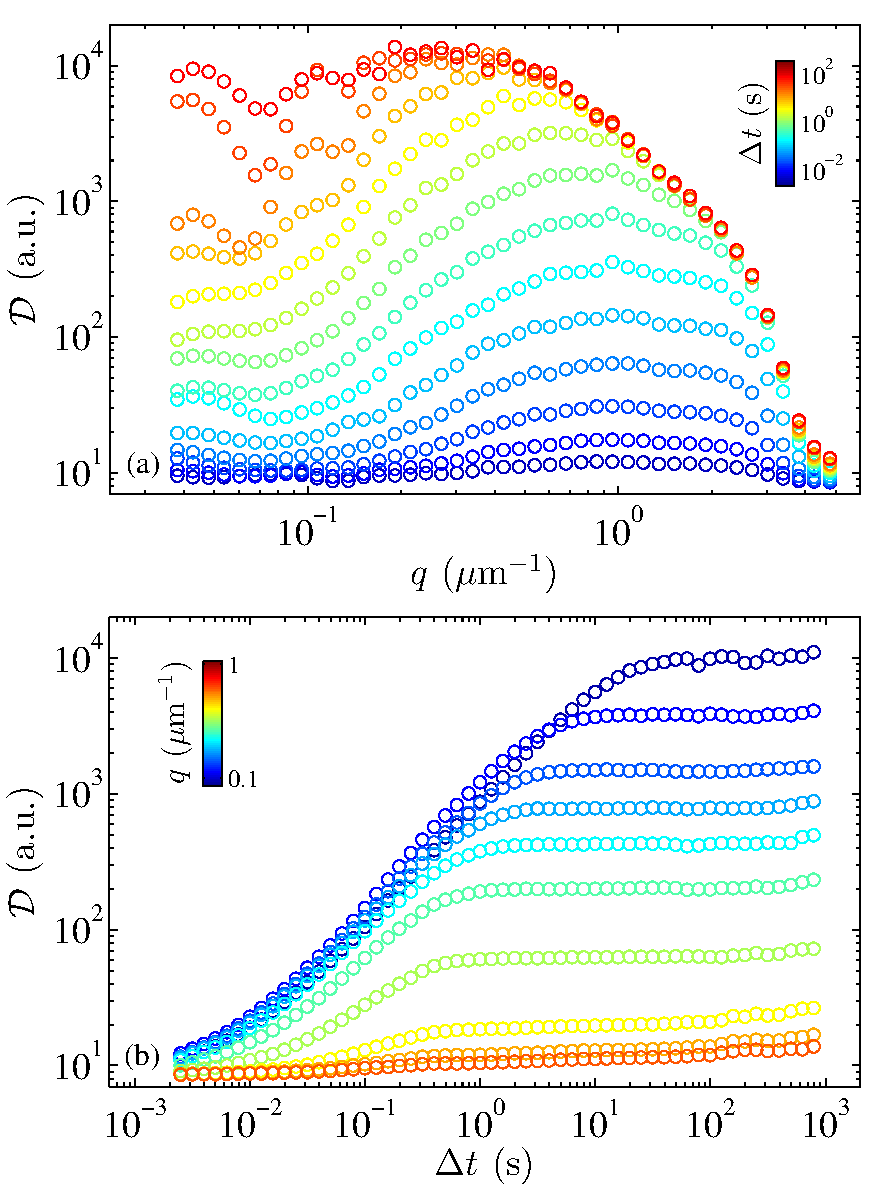
\includegraphics[width=\linewidth]{D_fonction_q_et_Deltat.pdf}\\
	\caption{Evolution of the Fourier transforms $\langle \, |\widehat{\Delta I}|^2 \, \rangle (q, \Delta t)$ of the differences of images as a function of the the wave vector $q$ calculated at various $\Delta t$ (a) and as a function of $\Delta t$ calculated at various $q$ (b).}
	\label{D}
\end{figure}

For each $q$ we fitted $\mathcal{D}(q, \Delta t)$ as a function of $\Delta t$. Our fit parameters are $A(q)$, $B(q)$ and $\tau_\text{d}(q)$. We fit the data in logarithmic scale in order not to attribute too much weight on points with high intensity and we dismiss timescales above 200 s where the statics is poor. The initial parameters for the fit are:
\begin{equation}
\left\{
\begin{array}{rcl}
A_0 &=& \mathcal{D} (q,\Delta t_\text{max}) - \mathcal{D} (q,\Delta t_\text{min}) \\
B_0 &=& \mathcal{D} (q,\Delta t_\text{min}) \\
\tau_\text{d} &=& \SI{1}{\second}
\end{array}
\right.
\end{equation}
where $\Delta t_\text{max}$ and $\Delta t_\text{min}$ are respectively the maximum and the minimum interval of time between two images.

Using the fit results for $A(q)$ and $B(q)$, we obtain the ISF, Fig.\ref{ISF}.a. According to (Eq.~\ref{eq:D2f}), by plotting $f(q, \Delta t)$ as a function of $\Delta t q^2$, we should remove every dependence of the ISF on $q$ resulting into a collapse of the data on a master curve. Indeed, this is what we observe in Fig.\ref{ISF}.b. 

%fig 6%%%%%%%%%%%%%%%%%%%%%%%%%%%%%%%%%%%%%%%
\begin{figure}
	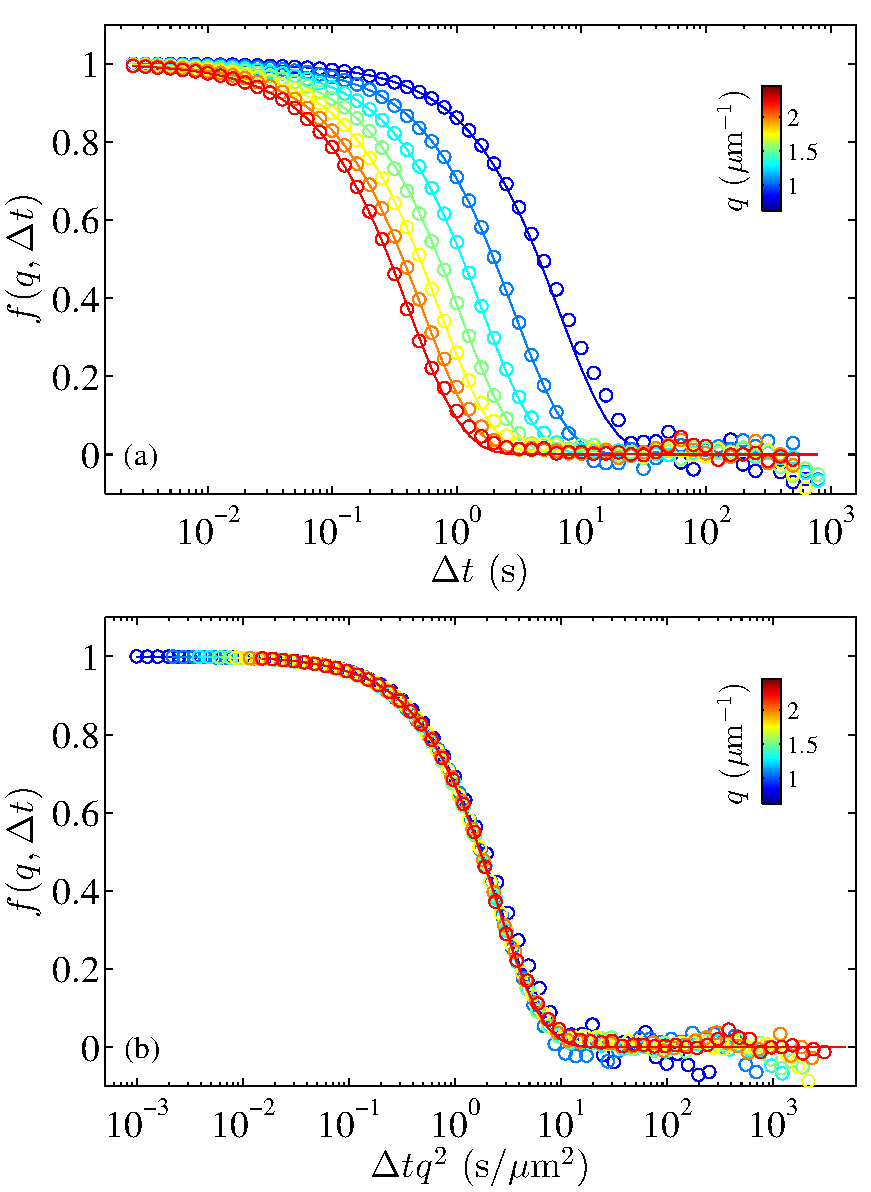
\includegraphics[width=\linewidth]{ISFColloides.pdf}\\
	\caption{Intermediate scattering function (ISF) calculated at various $q$ versus $\Delta t$ (a) and $\Delta tq^2$ (b). Lines are exponential fits to the data.}
	\label{ISF}
\end{figure}

When plotting the fitting parameters as a function of $q$, 3 regimes are visible,  Fig.\ref{FitDiffColl}:
\begin{itemize}
\item[\textbf{(1)}] Insufficient statistics. The radial average is performed on very few pixels (4 pixels for $q = q_\text{min}$ which correspond to the central cross of the Fourier transforms).  Also, at small $q$ the characteristic time is comparable to the duration of the experiment, $\SI{1000}{\second}$.
\item[\textbf{(3)}] For  $q>\SI{3.5}{\per\micro\meter}$, $A(q)$ (signal) is too close to $B(q)$ (noise), to yield a consistent fit. This sets the spatial resolution of DDM to  $\frac{2\pi}{3.5} = \SI{1.8}{\micro\meter}$.
\item[\textbf{(2)}] Statistics are good and the signal-to-noise ratio is low enough.
\end{itemize}

We fit $\tau_\text{d}(q)$ in regime (2) according to (Eq.~\ref{eq:relax}), which corresponds in logarithmic scale to a straight line of slope -2 and of intercept $-\log(D)$, Fig.\ref{FitDiffColl}.a. The theoretical model is in a very good agreement with our measurements and we obtain a diffusion coefficient of $D_\text{fit} = \SI{0.39}{\micro\meter\squared\per\second}$. Using the Stokes-Einstein formula with our experimental conditions, Table \ref{TabParams}, we obtain $D_\text{E} = \SI{0.41}{\micro\meter\squared\per\second}$ which implies an error of only $\sim 5 \%$. 


We also have access to informations about the parameters $A(q)$ and $B(q)$ , Fig.\ref{FitDiffColl}.b. According to our data, the noise level $B(q)$ seems constant for every $q$: the camera is adding a white noise to each images. With bright field, due to the depth of field of the objective in the $z$-direction, we are imaging a volume projected on $xy$ plane. The effect of the depth of field mostly affect the large length scales (small $q$) due to the disappearance of particles from the $z$-field and lead to underestimate the dynamics characteristic times\cite {4_Martinez20121637}. Taking into account the 3D nature of the experiment,  F.Giavazzi et al.\citep{3_DDM3D} have shown that it is possible to model $A(q)$.

%fig 7%%%%%%%%%%%%%%%%%%%%%%%%%%%%%%%%%%%%%%%
\begin{figure}
	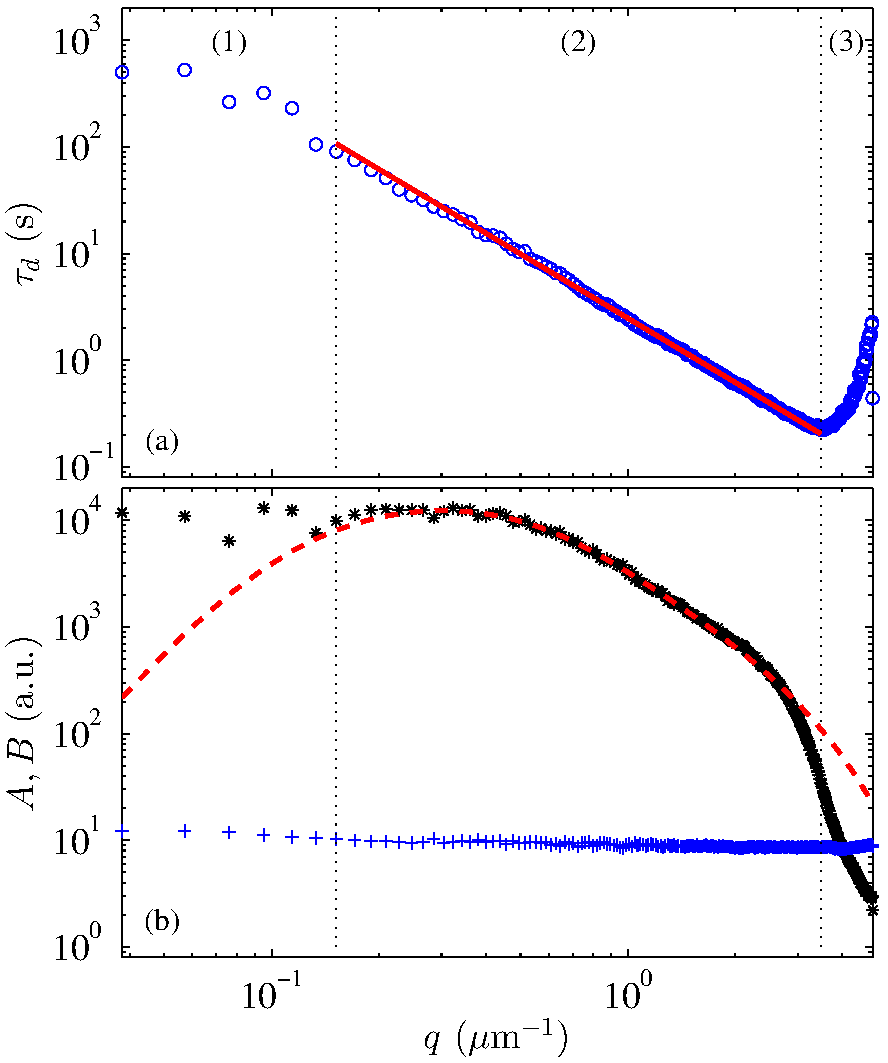
\includegraphics[width=\linewidth]{DiffusionColloids.pdf}\\
	\caption{Caracteristic brownian diffusion time and fit parameters A(q), B(q).(a) Experimental data (\textcolor{blue}{$\circ$}) and fitted curve (\textcolor{red}{\textbf{---}}) of the caracteristic time for brownian diffusion $\tau_\text{d}$ versus $q$. (b) Fit parameters A(q) ($\ast$), B(q) (\textcolor{blue}{+}), and a model for A(q) (\textcolor{red}{- -}). }
	\label{FitDiffColl}
\end{figure}

In this section, we have verified and dissected the DDM procedure. We have shown that we obtain via the intermediate scattering function quantitative information on the 3D dynamics of a hundreds of colloidal particles simultaneously on length scales ranging from $\sim \SI{2}{\micro\meter}$ to $\sim \SI{200}{\micro\meter}$ and on time scales ranging from the millisecond to the minutes. This exact experiment can also be exploited in a different manner thanks to the Stokes Einstein formula. Provided  that we know the temperature $T$ and the hydrodynamics radius of the colloids $r$, we can measure the viscosity of the solvant $\eta$.  Compared to a classical rheology experiment, DDM is actually better suited to measure small viscosity ($\sim$ mPas) of a solvent that we have on limited quantities ($\sim$ 50 $\mu L$). Finally, provided that this time we know $T$ and $\eta$, we can measure $r$ for particles size ranging from tens of nanometers to a few microns \cite{2_DDM}. Given the robustness and high throughput of DDM, DDM is appropriate for screening purposes.

\section{Bacteria and DDM}
\label{sec:BactSection}

\subsection{Bacteria}

The swimming of bacteria has been first observed in the 17th century with light microscopy by Antony van Leeuwenhoek \citep{23_dobell1933antony}, those bacteria are now known as \textit{Spirillum volutans}. However, he couldn't explain how they were moving as he was not able to see their propellant, the flagella, discovered only in 1836 by Christian Ehrenberg and also in 1872 by Ferdinand Cohn \citep{24_gillen2007genesis}. Then, biologists tried to understand how the bacteria was adapting the motion of their flagella to move in one given direction.
Nowadays, we know that the flagellum of bacteria is made of a set of multiple biological reversible rotary motors, a long helical filament, which serve as a propeller, and a coupler between the motors and the filament \citep{25_delalez2001bacterial}. The global motion of the bacteria can be split into two modes. In the ``tumble'' mode, the motors run clockwise and independently, causing the bacteria to move erratically. In the ``run'' mode, the motors run counter-clockwise but with the filaments rotating in parallel leading the bacteria to move ballistic and straight forward. A mean tumble has an average time of $\SI{0.1}{\second}$ and a run has an average time of $\SI{1}{\second}$ \citep{5_berg2000motile}. Both modes are exponentially distributed. The direction taken after a tumble is approximately random but there is a small bias due to the fact that bacteria are preferably moving toward a more nutritive medium. Bacteria chose their direction by comparing the variation of concentration over time \citep{26_mitchell2006bacterial}.

Bacteria are more complex particles than colloids. They are still sensitive to the thermal energy $k_\text{B}T$ but they also have their own source of energy and they ``run and tumble". With the same algorithm used with the Brownian particles, we study the global motion of bacteria. By adapting the functional form of the correlation function, we can disentangle diffusive from ballistic motion \citep{4_Martinez20121637}. We chose a specie of bacteria called \textit{Salmonella}. It has the shape of a rod with a length of $\SI{2}{\micro\meter}$ and a diameter of around $\SI{1}{\micro\meter}$. We chose this species of bacteria because, within the set of bacteria species we have tested, they displayed the highest motility ratio.

\subsection{Results}

Bacteria move preferably where the concentration of nutriments is higher, causing a bias in the direction taken after a tumble. As we gently mixed the culture medium during growth, the nutriment medium can be considered homogeneous in our samples and the bacteria are moving isotropically. We used the same acquisition parameters as with the colloids and applied the same algorithm as the one presented above. Contrary to the colloidal case, $f(q, \Delta t)$ shows a two step decay which corresponds to two decorrelation mechanisms, Fig.\ref{ISFBacteria}.a. We first identify the physical origin of those mechanism by trying a scaling approach. The first decorrelation mechanism, for $\Delta t < \SI{0.3}{\second}$, is due to a ballistic motion of bacteria. It is confirmed as the first decay of $f$  for different $q$  collapses on a master curve as we scale $f$ with the abscissa  $\Delta t q$ (dimension of an inverse velocity), see Fig.\ref{ISFBacteria}.b. The second decorrelation mechanism is due to a diffusion process and confirmed by the collapse of the second decay of $f$ for different $q$ when plotted as a function of $\Delta t q^2$ (dimension of an inverse diffusion coefficient), see Fig.\ref{ISFBacteria}.c.

Based on the scalings properties of the ISF, we turn to a model that takes into account:

\begin{itemize}
\item The Brownian motion of bacteria due to $k_BT$.
\item The mean velocity and the velocity distribution during the run.
\item The fact that some of our bacteria are motile and some are not.
\end{itemize}

Considering these new conditions, it can be shown that an adequate ISF is \citep{1_BactMobil}:
\begin{align}
f(q, \Delta t) &= \exp\left(-\frac{\Delta t}{\tau_\text{d}}\right)
\left[(1-\alpha) + \alpha \mathcal{P}(q, \Delta t)\right],\\
\mathcal{P}(q, \Delta t) &= \int_{0}^{\infty} P(v)\, \text{sinc}(q\, v\, \Delta t) \mathrm{d}v,
\end{align}
with $\tau_\text{d} = 1/(Dq^2)$ the characteristic Brownian diffusion time, $\alpha$ the fraction of motile bacteria. $\text{sinc}(q\, v\, \Delta t)$ is the ISF of an isotropic population of swimmers at velocity $v$. The distribution of velocity $P(v)$ and the integral $\mathcal{P}(q, \Delta t)$ over $v$ take into account that all bacteria do not move at the same velocity. 

Following Wilson et al.\cite{1_BactMobil}, we chose a Schulz distribution for $P(v)$ which respects the apparent dynamic of bacteria, i.e. peaked around the average velocity and going to 0 when $v \rightarrow \infty$:
\begin{multline}
P(v) = \frac{v^Z}{Z!} \left(\frac{Z+1}{\overline{v}}\right)^{Z+1} \exp\left[-\frac{v(Z+1)}{\overline{v}}\right],
\end{multline}
with $\overline{v}$ the mean velocity of bacteria.

It is then possible to formally calculate the integral over $v$:
\begin{multline}
\mathcal{P}(q, \Delta t) = \frac{(Z+1)\tau_\text{r}}{Z \, \Delta t} \sin\left(Z\tan^{-1}\left(\frac{\Delta t}{(Z+1)\tau_\text{r}}\right)\right)\\
\times \left(1+\left(\frac{\Delta t}{(Z+1)\tau_\text{r}}\right)^2\right)^{Z/2},
\end{multline}
with $\tau_\text{r} = 1/(\overline{v}q)$ the characteristic run time of bacteria and $Z$ is a parameter related to the standard deviation $\sigma$ of the distribution : $Z = \left( \frac{\overline{v}}{\sigma} \right)^2 -1$. 

Fitting $\mathcal{D}(q, \Delta t)$ requires 6 parameters, even though the 2 decays are well separated in time, we have initialized the fit with values very close to the results so that the fit converges:
\begin{equation}
\left\{
\begin{array}{rcl}
A_0 &=& \mathcal{D} (q,\Delta t_\text{max}) - \mathcal{D} (q,\Delta t_\text{min}) \\
B_0 &=& \mathcal{D} (q,\Delta t_\text{min}) \\
\tau_\text{d0} &=& 1/(0.1 q^{2})\\
\alpha_0 &=& 0.5\\
\tau_\text{r0} &=& 1/(10 q)\\
Z_0 &=& 1
\end{array}
\right.
\end{equation}


%fig 8%%%%%%%%%%%%%%%%%%%%%%%%%%%%%%%%%%%%%%%
\begin{figure}
	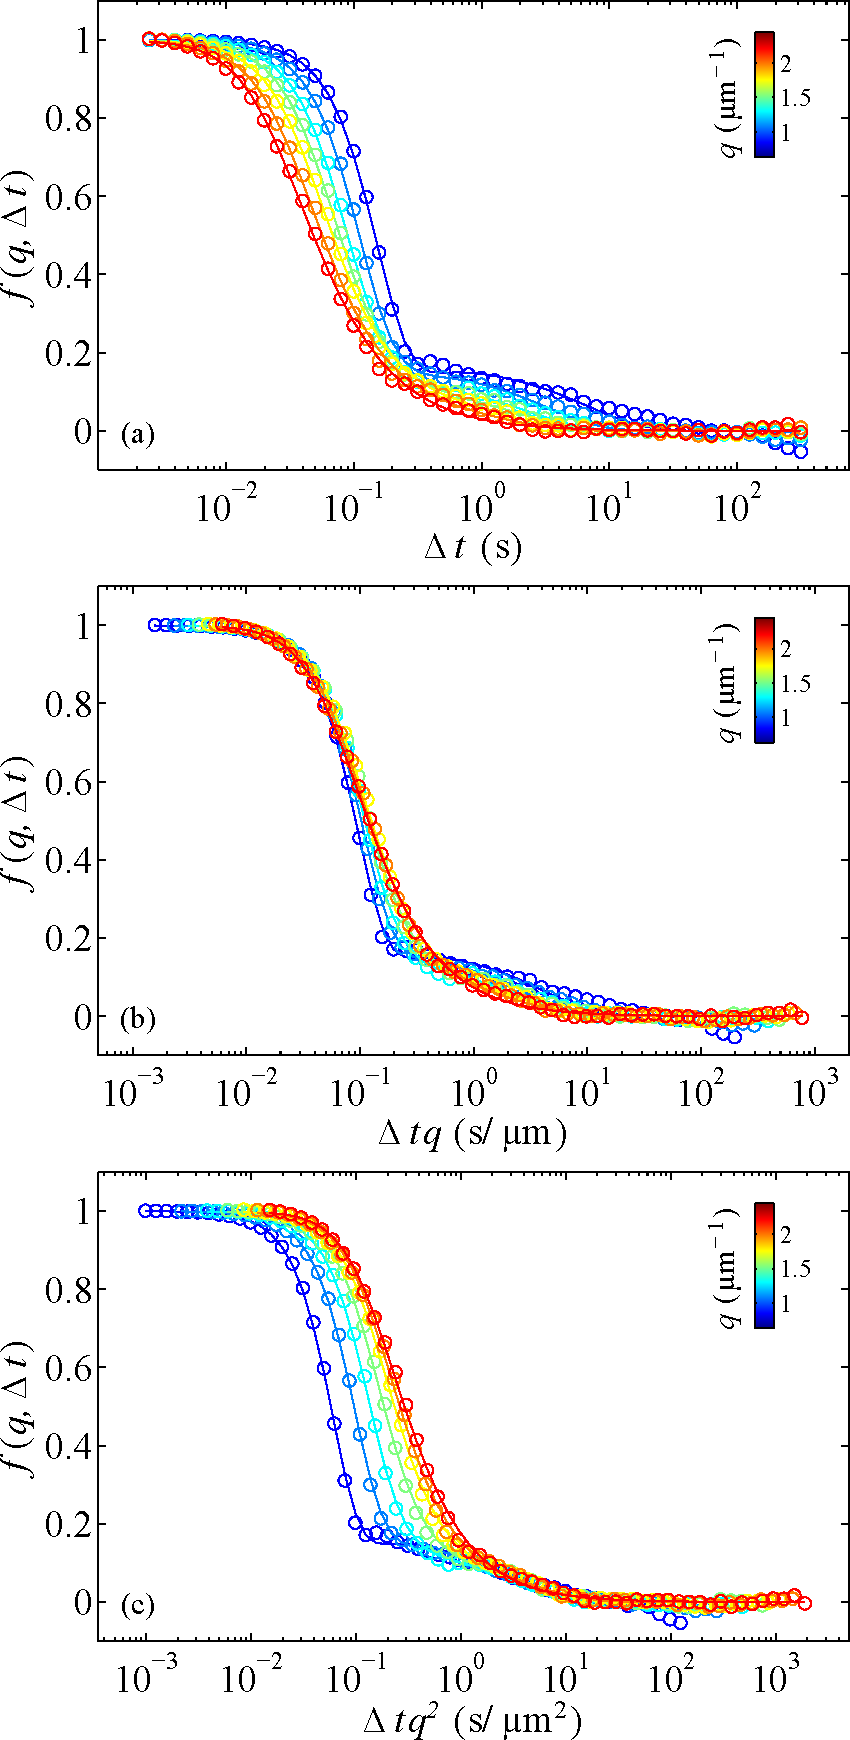
\includegraphics[width=\linewidth]{ISF_Fonction_TetTq2etTq_Bact.pdf}\\
	\caption{Intermediate scattering function (ISF) calculated at various $q$ versus $\Delta t$ (a), $\Delta tq$ (b) and $\Delta tq^2$ (c). Lines are fit to the data.}
	\label{ISFBacteria}
\end{figure}

Fitting parameters are displayed in Fig. \ref{FitParametersBacteria} function of $q$. We limit the $q$ range to the regime (2) set by the colloid experiment where the statistics and the signal to noise are optimal. The run time and the diffusion time can be reasonably fitted in logarithmic scale by straight lines of respective slopes -1 (ballistic) and -2 (diffusion) whose respective intersects yield $\overline{v} = \SI{21.2}{\micro\meter\per\second}$ with the Shultz distibution characterized by a standard deviation of $\sigma=\SI{11.3}{\micro\meter\per\second}$ and $D = \SI{0.28}{\micro\meter\squared\per\second}$. The \textsc{Stokes-Einstein} relation considering spherical bacteria of diameter $\SI{1.5}{\micro\meter}$, a viscosity $\eta = \SI{1}{\milli\pascal\second}$ and a temperature $T=\SI{293}{\kelvin}$, yields $D_\text{SE} = \SI{0.28}{\micro\meter\squared\per\second}$, a very good agreement even though we are not considering the real shape of bacteria. Our bacteria suspension displays a high fraction of motile bacteria, $\alpha\approx$ 0.8 and are quite fast compared to E. Coli ($\alpha\approx 0.6$, $\overline{v} \approx \SI{10}{\micro\meter\per\second}$)\cite{4_Martinez20121637}. $\alpha$, $Z$ and $\sigma$ are expected to be constant as the statistical properties of the bacteria dispersion should not change over the duration of the experiment. This is roughly what we observe.

In the model and our experiment we are not characterizing tumble. On the experimental side, this would require to measure over a much longer time. On the theoretical side, Martens et al. \cite{6_martens2012probability} have proposed a model for the ISF that takes into account the tumble.

%fig 9%%%%%%%%%%%%%%%%%%%%%%%%%%%%%%%%%%%%%%%
\begin{figure}
	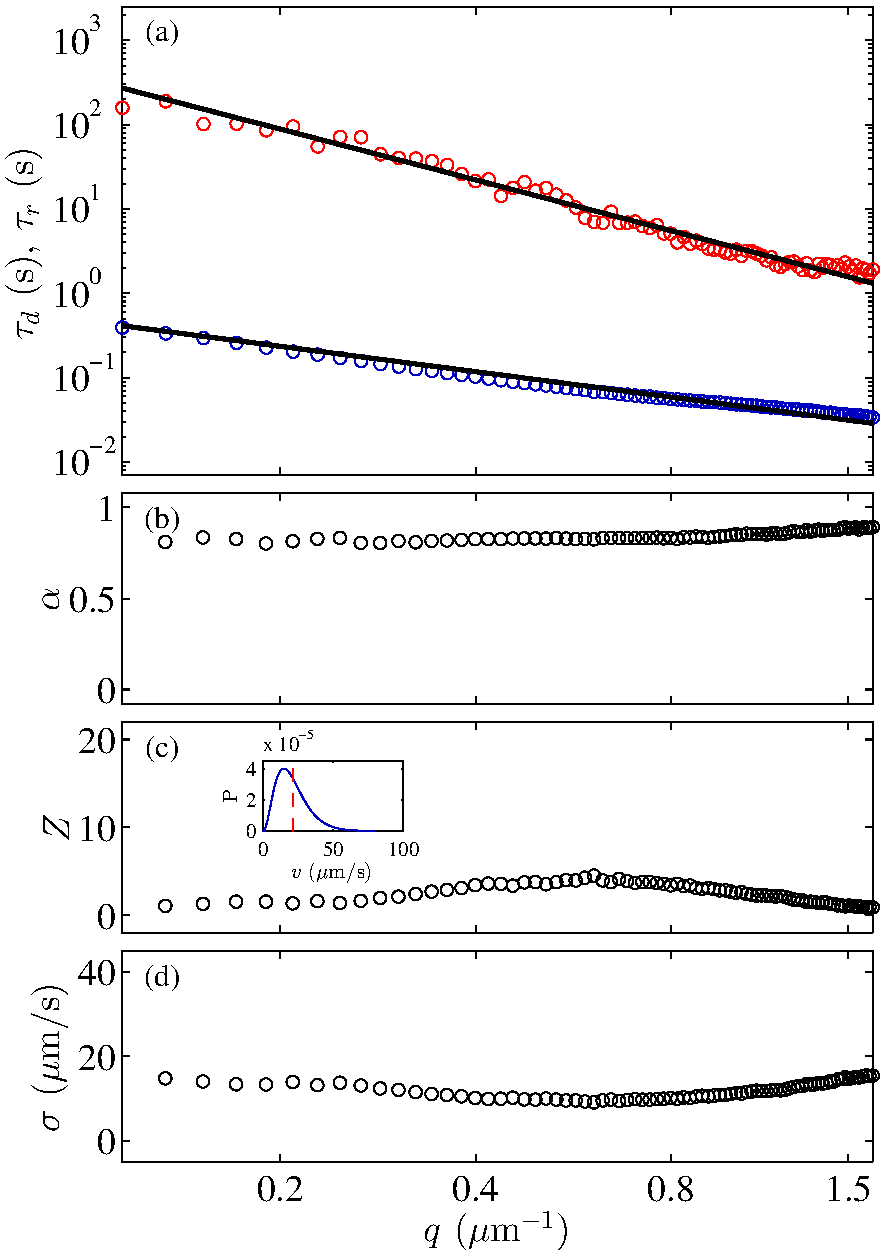
\includegraphics[width=\linewidth]{VitesseDiffusionParams.pdf}\\
	\caption{Fit parameters for the motile bacteria as a function of $q$. (a) characteristic time for the diffusion, $\tau_d$, and balistic motion, $\tau_r$. (b) Fraction of motile bacteria $\alpha$. (c) $Z$. Inset: Shulz velocity distribution, $P$ for $<Z>$=2.4. (d) Standard deviation of the Shulz distribution, $\sigma$.}
	\label{FitParametersBacteria}
\end{figure}

\section{\label{cl}Conclusion}

Differential Dynamics Microscopy (DDM) is a microscopy technique that probes the dynamics of a system of particles using a microscope, a camera and numerical computations. We exposed this technique in the well-known case of simple Brownian motion before applying it to the more complex case of motile bacteria. We have shown how to extract physically relevant information from DDM based on scaling and how to obtain quantitative values such as the diffusion coefficient or the velocity..

DDM is based  on microscopy and can therefore benefit from  more advanced techniques than bright field imaging. For example, it is possible to use fluorescence microscopy to tell apart colloidal probes in a crowed medium\cite{Hendricks2015}, confocal microscopy\cite{Lu2012}, or polarized light microscopy\citep{20_reufer2012differential}. Apart from colloidal Brownian motion and bacteria, DDM has also been used to characterize ellipsoidal particles\citep{20_reufer2012differential} and kinetics of phase separation\cite{Gao2015} and aggregation\cite{Ferri2011}. Even macroscopic systems, like human crowds shot from above, could be studied by DDM. In that sense, DDM opens much more possibilities than dynamic light scattering and can be used in various contexts both in the lab and in the classroom.

\section*{\label{epaps}EPAPS}
\begin{itemize}
 \item Movie 1: bright field stack composed of 4000 images of colloidal particle dispersed in water. $f_{acq}=400$ Hz. $\SI{1}{px} = \SI{0.645}{\micro\meter}$. Image size = $(\SI{512}{px})^2$.
 \item Movie 2: bright field stack composed of 4000 images of colloids dispersed in water. $f_{acq}=4$ Hz. $\SI{1}{px} = \SI{0.645}{\micro\meter}$. Image size = $(\SI{512}{px})^2$.
 \item Movie 3: bright field stack composed of 4000 images of $salmonella$ bacteria dispersed in water. $f_{acq}=400$ Hz. $\SI{1}{px} = \SI{0.645}{\micro\meter}$. Image size = $(\SI{512}{px})^2$.
 \item Movie 4: bright field stack composed of 4000 images of $salmonella$ bacteria dispersed in water. $f_{acq}=4$ Hz. $\SI{1}{px} = \SI{0.645}{\micro\meter}$. Image size = $(\SI{512}{px})^2$.
 \item DDM code in Matlab.
 \item DDM code in Python.
\end{itemize}

\begin{acknowledgments}
The authors would like to thank the students who endured the initial versions of this lab work: Alicia Damm, Florine Dubourg, D.G. himself, Paul Haddad, Gabriel Rigon and Sylvie Sue. Fig.~\ref{Slide} and \ref{BrownianTrajectory} where adapted from the work of J\'er\'emy Ferrand and Paco Maurer~\cite{Maurer2014}. 
This work was supported by the ENS Lyon, the Agence Nationale de la Recherche fran\c{c}aise (ANR-11-PDOC-027) and PALSE XXX.
\end{acknowledgments}

\bibliographystyle{unsrt}
\bibliography{./DGermain_2015bib}


\end{document}
